\documentclass[border={7pt 0pt 7pt 0pt},varwidth]{standalone}
\usepackage{amsmath}
\usepackage[dvipsnames]{xcolor}%colors
\usepackage{tikz-cd,tikz-3dplot} 
\usepackage{diagbox}
\usepackage{makecell}
\usepackage{adjustbox}
\usepackage{multirow}
\usepackage[width=0.5,tiewidth=0.7]{strands}
\usepackage{array}

\newcommand{\fakestar}{*}
\begin{document}
\begin{table}[]
\arraycolsep=1pt
\[
 \setcellgapes{0ex}\makegapedcells
\begin{array}{ccccccccccc}

    \;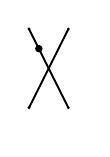
\begin{tikzpicture}[baseline=(current bounding box)]
    \tie[color=black,bull=1,bulletie=0.01,style=solid]{{2,1},{1,0}}
    \tie[color=black,bull=1,bulletie=0.01,style=solid]{{1,1},{2,0}}
    \tie[color=black]{{1.25,0.75}}
    \node at (0.5,-0.07) {$\phantom{\scriptstyle i}$};
    \end{tikzpicture}        &=&
    \;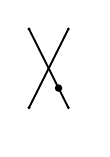
\begin{tikzpicture}[baseline=(current bounding box)]
        \tie[color=black,bull=1,bulletie=0.01,style=solid]{{2,1},{1,0}}
        \tie[color=black,bull=1,bulletie=0.01,style=solid]{{1,1},{2,0}}
        \tie[color=black]{{1.75,0.25}}
        \node at (0.5,-0.07) {$\phantom{\scriptstyle i}$};
    \end{tikzpicture} &-&
\;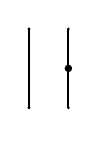
\begin{tikzpicture}[baseline=(current bounding box)]
        \tie[color=black,bull=1,bulletie=0.01,style=solid]{{1,1},{1,0}}
        \tie[color=black,bull=1,bulletie=0.01,style=solid]{{2,1},{2,0}}
        \tie[color=black]{{2,0.5}}
\node at (0.5,-0.07) {$\phantom{\scriptstyle i}$};
    \end{tikzpicture}        
        &\hspace{10mm}$\,$
        &\;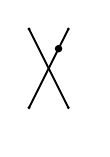
\begin{tikzpicture}[baseline=(current bounding box)]
            \tie[color=black,bull=1,bulletie=0.01,style=solid]{{2,1},{1,0}}
            \tie[color=black,bull=1,bulletie=0.01,style=solid]{{1,1},{2,0}}
            \tie[color=black]{{1.75,0.75}}
            \node at (0.5,-0.07) {$\phantom{\scriptstyle i}$};
    \end{tikzpicture}        &=&
            \;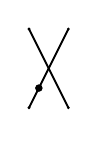
\begin{tikzpicture}[baseline=(current bounding box)]
                \tie[color=black,bull=1,bulletie=0.01,style=solid]{{2,1},{1,0}}
                \tie[color=black,bull=1,bulletie=0.01,style=solid]{{1,1},{2,0}}
                \tie[color=black]{{1.25,0.25}}
                \node at (0.5,-0.07) {$\phantom{\scriptstyle i}$};
    \end{tikzpicture} &+&
        \;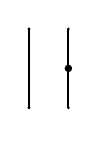
\begin{tikzpicture}[baseline=(current bounding box)]
                \tie[color=black,bull=1,bulletie=0.01,style=solid]{{1,1},{1,0}}
                \tie[color=black,bull=1,bulletie=0.01,style=solid]{{2,1},{2,0}}
                \tie[color=black]{{2,0.5}}
        \node at (0.5,-0.07) {$\phantom{\scriptstyle i}$};
    \end{tikzpicture} 
           \\
D_ie_i &=& e_{i+1}D_i &-&e_{i+1}& &    D_ie_{i+1} &=& e_{i}D_i &+&e_{i+1}\\
\\
    \;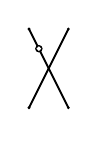
\begin{tikzpicture}[baseline=(current bounding box)]
    \tie[color=black,bull=1,bulletie=0.01,style=solid]{{2,1},{1,0}}
    \tie[color=black,bull=1,bulletie=0.01,style=solid]{{1,1},{2,0}}
    \tie[color=black]{{1.25,0.75}}
    \tie[color=white,bulletie=0.02]{{1.25,0.75}}
    \node at (0.5,-0.07) {$\phantom{\scriptstyle i}$};
    \end{tikzpicture}        &=&
    \;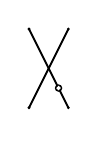
\begin{tikzpicture}[baseline=(current bounding box)]
        \tie[color=black,bull=1,bulletie=0.01,style=solid]{{2,1},{1,0}}
        \tie[color=black,bull=1,bulletie=0.01,style=solid]{{1,1},{2,0}}
        \tie[color=black]{{1.75,0.25}}
        \tie[color=white,bulletie=0.02]{{1.75,0.25}}
        \node at (0.5,-0.07) {$\phantom{\scriptstyle i}$};
    \end{tikzpicture} &+&
\;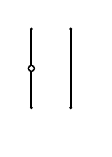
\begin{tikzpicture}[baseline=(current bounding box)]
        \tie[color=black,bull=1,bulletie=0.01,style=solid]{{1,1},{1,0}}
        \tie[color=black,bull=1,bulletie=0.01,style=solid]{{2,1},{2,0}}
        \tie[color=black]{{1,0.5}}
        \tie[color=white,bulletie=0.02]{{1,0.5}}
\node at (0.5,-0.07) {$\phantom{\scriptstyle i}$};
    \end{tikzpicture}        
        &\hspace{10mm}$\,$
        &\;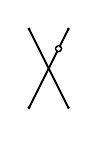
\begin{tikzpicture}[baseline=(current bounding box)]
            \tie[color=black,bull=1,bulletie=0.01,style=solid]{{2,1},{1,0}}
            \tie[color=black,bull=1,bulletie=0.01,style=solid]{{1,1},{2,0}}
            \tie[color=black]{{1.75,0.75}}
            \tie[color=white,bulletie=0.02]{{1.75,0.75}}
            \node at (0.5,-0.07) {$\phantom{\scriptstyle i}$};
    \end{tikzpicture}        &=&
            \;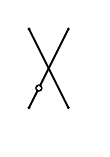
\begin{tikzpicture}[baseline=(current bounding box)]
                \tie[color=black,bull=1,bulletie=0.01,style=solid]{{2,1},{1,0}}
                \tie[color=black,bull=1,bulletie=0.01,style=solid]{{1,1},{2,0}}
                \tie[color=black]{{1.25,0.25}}
                \tie[color=white,bulletie=0.02]{{1.25,0.25}}
                \node at (0.5,-0.07) {$\phantom{\scriptstyle i}$};
    \end{tikzpicture} &-&
        \;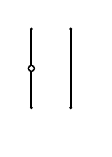
\begin{tikzpicture}[baseline=(current bounding box)]
                \tie[color=black,bull=1,bulletie=0.01,style=solid]{{1,1},{1,0}}
                \tie[color=black,bull=1,bulletie=0.01,style=solid]{{2,1},{2,0}}
                \tie[color=black]{{1,0.5}}
                \tie[color=white,bulletie=0.02]{{1,0.5}}
        \node at (0.5,-0.07) {$\phantom{\scriptstyle i}$};
    \end{tikzpicture} 
           \\
D_ie_i^{-1} &=& e_{i+1}^{-1}D_i &+&e_{i}^{-1}& &    D_ie_{i+1}^{-1} &=& e_{i}^{-1}D_i &-&e_{i}^{-1}\\
\\
\multicolumn{5}{c}{
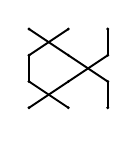
\begin{tikzpicture}[baseline=(current bounding box)]
            \tie[color=black,bull=1,bulletie=0.01,style=solid]{{3,1},{3,0.6667},{2,0.3333},{1,0}}
            \tie[color=black,bull=1,bulletie=0.01,style=solid]{{2,1},{1,0.6667},{1,0.3333},{2,0}}
            \tie[color=black,bull=1,bulletie=0.01,style=solid]{{1,1},{2,0.6667},{3,0.3333},{3,0}}
            \node at (0.5,-0.07) {$\phantom{\scriptstyle i}$};
\end{tikzpicture} \hspace{5mm}=\hspace{5mm} 
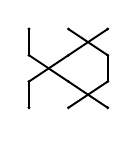
\begin{tikzpicture}[baseline=(current bounding box)]
            \tie[color=black,bull=1,bulletie=0.01,style=solid]{{3,1},{2,0.6667},{1,0.3333},{1,0}}
            \tie[color=black,bull=1,bulletie=0.01,style=solid]{{2,1},{3,0.6667},{3,0.3333},{2,0}}
            \tie[color=black,bull=1,bulletie=0.01,style=solid]{{1,1},{1,0.6667},{2,0.3333},{3,0}}
            \node at (0.5,-0.07) {$\phantom{\scriptstyle i}$};
\end{tikzpicture}\hspace{3.6mm}\;
} && \;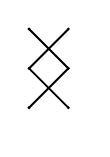
\begin{tikzpicture}[baseline=(current bounding box)]
            \tie[color=black,bull=1,bulletie=0.01,style=solid]{{1,1},{2,0.5},{1,0}}
            \tie[color=black,bull=1,bulletie=0.01,style=solid]{{2,1},{1,0.5},{2,0}}
            \node at (0.5,-0.07) {$\phantom{\scriptstyle i}$};
    \end{tikzpicture}        &=&
            \;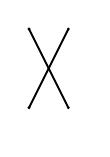
\begin{tikzpicture}[baseline=(current bounding box)]
                \tie[color=black,bull=1,bulletie=0.01,style=solid]{{2,1},{1,0}}
                \tie[color=black,bull=1,bulletie=0.01,style=solid]{{1,1},{2,0}}
                \node at (0.5,-0.07) {$\phantom{\scriptstyle i}$};
    \end{tikzpicture}\\
    \multicolumn{5}{c}{
    D_iD_{i+1}D_i \;=\; 
    D_{i+1}D_iD_{i+1}
    }&& D_i^{2}&=&D_i
\end{array}
\]
\end{table}
\end{document}